\section{Application case: Pacer}
	\label{sec:pacer}
	
	\par \textbf{Pacer: Pedometer \& Step Tracker} is one of the most downloaded applications among the \textit{Health \& Fitness} apps. Developed by \textit{Pacer Health} it counts more then 10 Millions downloads and almost 900 thousands reviews. It delivers pedometer and exercise tracking services. The application let the user create his own profile delivering detailed statistics on his fitness activity. The registration of a new account is mandatory to use the application. \newline
	\par The network communication protocol has been analyzed using both HttpToolkit and BurpSuite. Moreover the tool Frida has been useful for runtime instrumentation, and the GDA tool has been used for static analysis. 
	\par The investigation of this application lead in fact, to some important vulnerabilities discovery. All the details are covered in the next section.
	
	\subsection{Study detail}	
		\par After having installed the application on the Android emulator, Pacer has been investigated throughout its entire runtime, with the HttpToolkit software as proxy in order to intercept the encrypted traffic.\newline
		All the research plan and workflow is described step-by-step in the following paragraphs.
		
		\subsubsection{New account setup}
			\par At the moment of creating a new account, multiple POST and PUT requests are issued towards the \textit{log.pacer.cc} endpoint. A new session of the user, still unauthenticated, is created. In the first request are sent \textit{app\_version} and \textit{device\_id} as parameters, and the response will contain the information about the session just created. At this point the user can start the procedure to create a new Pacer account, by typing in the application some information on his person. From the technical point of view two different resources are accessed:
			\begin{enumerate}
				\item \textit{/pacer/android/api/v18/accounts/334794565/devices}: This resource contains the informations about the devices used to access that specific account. The body of the request looks like the following:
\begin{lstlisting}
POST /pacer/android/api/v18/accounts/334794565/devices

app_version=p9.10.2
device_id=7021f2bad994fb65
device_model=sdk_gphone64_x86_64
sim_country_code_iso=us
push_service=gcm
platform=android
app_name=cc.pacer.androidapp_play
rom=5.15.41-android13-8-00205-gf1bf82c3dacd-ab8747247%288808248%29
platform_version=13
app_version_code=2022102700
payload=
device_token= <device_token>
has_blood_pressure=false
has_heart_rate=false
has_weight=true
\end{lstlisting}
				\item \textit{/pacer/android/api/v18/accounts/334794565}: This resource contains all the informations about the user account. Initially a POST request is issued to create the resource and a subsequent PUT request will add information on the resource. Here is reported the body of the final PUT request.
\begin{lstlisting}
PUT /pacer/android/api/v18/accounts/334794565

avatar_name=sports_running
avatar_path=
display_name=PacerPal
first_install_device_uuid=d9132b20-6a9f-4486-be1f-713a21f113f7
gender=male
language=en
locale=en_US
login_id_alias=p334794565
sim_country_code_iso=us
source=pacer_android
timezone=GMT
timezone_offset_in_minutes=0
unit_type=metric
year_of_birth=1996
\end{lstlisting}
			\end{enumerate} 
			
			\par At this point the user is asked to link his fresh Pacer account to Google and Facebook as identity provider. This will automatically fill in informations like \textit{avatar\_path} and \textit{display\_name}. If the user agrees, a new PUT request on the same \textit{/pacer/android/api/v18/accounts/334794565} resource is issued. The body values are the same, but with additional specifications for \textit{avatar\_path} and \textit{display\_name}:
\begin{lstlisting}
PUT /pacer/android/api/v18/accounts/334794565

	avatar_name=sports_running
+	avatar_path= image path from <googleusercontent.com>
	content_generated_by=user
+	display_name=Nicola
	first_install_device_uuid=d9132b20-6a9f-4486-be1f-713a21f113f7
	gender=male
	language=en
	locale=en_US
	login_id_alias=p334794565
	sim_country_code_iso=us
	source=pacer_android
	timezone=GMT
	timezone_offset_in_minutes=0
	unit_type=metric
	year_of_birth=1996
\end{lstlisting}
			\par The account creation and social linking service is done. The Pacer service already got all the information needed to let the user start using the application.
	
		\subsubsection{Application startup}
		\par The Pacer application is ever running in background, even if the application is being closed or minimized. Everytime the application transitions from the background to the foreground (passing to the top of the screen), a POST request is issued towards the \textit{log.pacer.cc} endpoint. The \textit{app\_in\_foreground} action is communicated to the server together with \textit{app\_version} and \textit{device\_id} as parameters, and \textit{account\_id} and \textit{install\_days} as body fields:
\begin{lstlisting}
POST /pacer/android/api/v18/accounts/334794565/actions/app_in_foreground?app_version=p9.10.2&device_id=7021f2bad994fb65

account_id=334794565
action=app_in_foreground
install_days=
\end{lstlisting}
		\par This request that, up to now, does not provide any useful information. But it is something that we will be using later on in the investigation.
		
		\subsubsection{Accessing resources}
			\par After having fully configured the account the user can start using the application. Most of the interaction is done towards the server \textit{api.pacer.com} responsible for delivering the services implemented by the application, while few interactions related to logging purposes are directed towards \textit{log.pacer.cc}. \newline
			When the user opens the application, he will be showed the homepage containing informations related to his daily activity. At the same time the informations on his account will be retrieved from the Pacer server. Since in the study we are interested in the personal user information, I will explain how these data are obtained. \newline
			There are two ways in which the application gathers the information associated to a specific \textit{pacer\_id} Pacer account:
			\begin{enumerate}
				\item If the target \textit{pacer\_id} is the one associated to the user currently using the application, then a GET request is issued on the resource \textit{/pacer/android/api/v18/accounts/<pacer\_id>}. This is the request issued when the user opens up the application, visiting the main page of the application. The body of the response is a JSON structure containing the following data (some informations cutted off for length reasons):
\begin{lstlisting}
{
  "id": 334794565,
  "login_id": "p334794565",
  "info": {
    "avatar_name": "sports_running",
    "avatar_path": "https://lh3.googleusercontent.com/a/ALm5wu2j-G2Ncb9yct7pyxZr1RuD9UmxVldbgh_BO3MULw=s96-c",
    "display_name": "Nicola",
    "gender": "male",
    "year_of_birth": 1996,
    "source": "pacer_android",
    "email": "alocinalocin@gmail.com",
    "email_status": "active",
    "has_password": false,
    "first_install_device_uuid": "B762315C-EFC0-44BA-9CF8-4CF11534D926"
  },
  "settings": {
    "privacy_type": "private"
  },
  "social": [
    {
      "id": 80332936,
      "social_id": "102620851772027851844",
      "social_id_internal": "102620851772027851844_st_google",
      "head_img_url": "https://cdn.pacer.cc/accounts/334794565/images/avatar/2022/11/334794565_af56c5f9-5a23-49f7-ba85-f50087bacdff_1668006978150.jpg",
      "nick_name": "Nicola",
      "social_type": "google"
    },
    {
      "id": 80405740,
      "social_id": "5495598560535308",
      "social_id_internal": "5495598560535308_st_fb",
      "head_img_url": "https://platform-lookaside.fbsbx.com/platform/profilepic/?asid=5495598560535308&height=50&width=50&ext=1671029057&hash=AeRZcSELt4mZ1V-t9aQ",
      "nick_name": "Nicola Iommazzo",
      "social_type": "fb"
    }
  ],
  "follower_count": "1",
  "following_count": "1"
}
\end{lstlisting}
				These are the informations retrieved by the Pacer server on our specific account, in fact since we are the owner of the account we have the permissions to view some personal informations like the \textit{email} associated to the account and the whole \textit{social} section containing the reference to our Facebook and Google accounts.
				\item If an user would like to visit the profile of a different \textit{pacer\_id} Pacer user profile the request issued is slightly different. A GET request is made towards the resource \textit{/pacer/android/api/v18/accounts/335041780/profile} passing as parameters: \newline \textit{visitor\_account\_id=334794565\&sim\_country\_code\_iso=us}. \newline
				This is the request generated for example when the user wants to visit a profile from his friends list. Since we are visiting an account that we do not own the information retrieved will be less accurated. The JSON response obtained is:
\begin{lstlisting}
{
  "success": true,
  "status": 200,
  "data": {
    "id": 335041780,
    "login_id": "k335041780",
    "settings": {
      "privacy_type": "public",
    },
    "info": {
      "id": 335011000,
      "avatar_name": "icon_dongdong",
      "avatar_path": "https://cdn.pacer.cc/img/avatar/light/04_12.png",
      "display_name": "iommazzo.1693395",
      "gender": "male",
      "year_of_birth": 1980,
      "account_id": 335041780,
      "source": "pacer_android"
    },
    "location": {
      "display_name": "Italy",
      "region_id": "country_it"
    },
    "following_count": "1",
    "follower_count": "1",
    "isPremium": false,
    "is_blocked_by_me": false,
    "social_relationship": "bifollowing",
    "follower_status": "active",
    "following_status": "active"
  }
}
\end{lstlisting}
				Among the informations retrieved there are not either the email or the social network fields.
			\end{enumerate}
			
			\par So basing on the fact that we are visiting our own account or a different user one, the two requests are generated automatically while using the application. But what is the behaviour of the application if we manually forge a request specifc for the first or second case? For example what happens if we use the first way of accessing resource (aimed to access our own account informations) but using a \textit{pacer\_id} different from the one of our account.
		
		\subsubsection{Testing unauthorized access \#1}
			\par For this case I used two different accounts, the first one is linked to the institutional email offered by Sapienza, while the second one is linked with my personal email. The first account with id \textit{335041780} is used to generate the requests; the second account with id \textit{334794565} is the target account. Goal of this test is to understand if it is possible to obtain informations on a different user account, with the same accuracy degree as we were retrieving our account informations. For this kind of tests I used the \textit{Repeater} feature implemented in the BurpSuite software, explained in section \ref{sec:burp_suite}. \newline
			\par The first test I tryed was to manually forge a GET request towards the second account resource. The idea is to use the first way of accessing resources but on a different \textit{pacer\_id} account. Starting from the standard request generated when visiting our account, I simply changed the path of the resource to \textit{/pacer/android/api/v18/accounts/334794565}:
			\begin{figure}[ht]
				\centering
				\subfigure[Request to own resource]{
				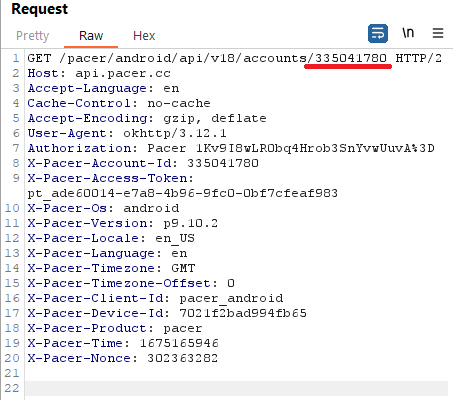
\includegraphics[width=.47\textwidth]{images/pacer1.png}
				}
				\subfigure[Request to different account resource]{
				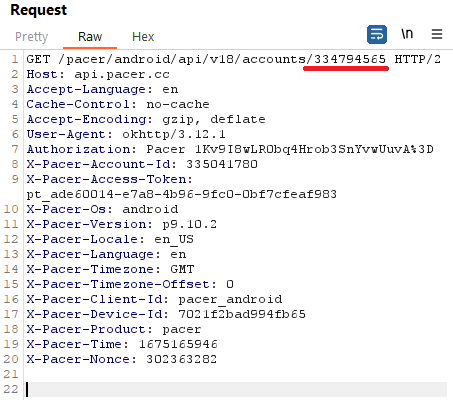
\includegraphics[width=.47\textwidth]{images/pacer2.png}
				}
				\caption{Test request \#1}
			\end{figure}
			\par The result is negative. The request in Figure 4.1(b) does not work, returning in the response the message: \newline
			\textit{\{"success":false,"code":500,"message":"Oops! Could not complete the requested operation, please try again later and contact support@mypacer.com if the error persists."\}}. \newline
			\par In any case the behaviour of the application can be understood by carefully reading the error message. It is saying that the request cannot be completed, meaning that maybe it is malformed. There is no message saying that we are unauthorized to access that resource.
			\par Looking at the header fields, there are multiple customized headers of the form \textit{X-Pacer-<value>}. Moreover there is an \textit{Authorization} header that definitely is important. By looking at two generated requests on HttpToolkit to the same resource there are three headers changing every time. \textbf{X-Pacer-Time}, \textbf{X-Pacer-Nonce} and \textbf{Authorization} headers are always different. Definitely those fields have to be coherent each other. 
			
		\subsubsection{The Authorization header}
			\par At this point I decided to explore more in depth how the \textit{Authorization} header is being computed. There are no particular requests the application is performing to retrieve that header everytime, so definitely it has to be computed at runtime by the application.\newline
			I started analyzing the \textit{.apk} file of the application in the \textbf{GDA} tool explained in Section \ref{subsec:gda}. With the search string feature provided by the tool, I looked for the string \textit{''Authorization''}, ending up on the following code:
			\begin{figure}[ht]
				\centering
				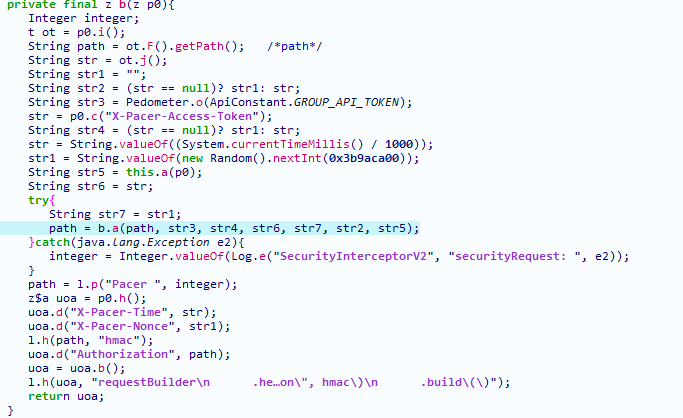
\includegraphics[width=0.7\textwidth]{images/pacer_gda1.png}
				\caption{Private method \textit{b}.}
			\end{figure}
			\par In this code I also found some other strings like \textit{''X-Pacer-Access-Token''}, \textit{''X-Pacer-Time''} and \textit{''X-Pacer-Nonce''}. The semantic of this method is pretty unknown up to now. In the highlighted line we can see that an additional method \textit{a} is called on the object \textit{b} passing as parameter some strings, and obtaining a value called \textit{path}. Looking at the code those strings are:
			\begin{itemize}
				\item \textit{str3} is obtained from the \textit{Pedometer} object; 
				\item \textit{str4} is equal to the \textit{X-Pacer-Access-Token}, if it is not \textit{null};
				\item \textit{str6} is equal to \textit{String.valueOf((System.currentTimeMillis() / 1000))};
				\item \textit{str7} is equal to \textit{String.valueOf((new Random().nextInt(0x3b9aca00)))}; 
				\item \textit{str2} is obtained from a structure \textit{ot}, if it is not \textit{null}; 
				\item \textit{str5} is obtained from \textit{this} object with the method \textit{a};
				\item \textit{path} is obtained from the method \textit{getPath()}.
				\item The same \textit{path} variable is also the return value of the method in the highlighted line. After in the code this variable is used along with the \textit{''Authorization''} string.
			\end{itemize} 
			I have also inspected the highlighted method \textit{a}, that is being called passing all the above strings as parameters. This is the relative code:
			 \begin{figure}[ht]
				\centering
				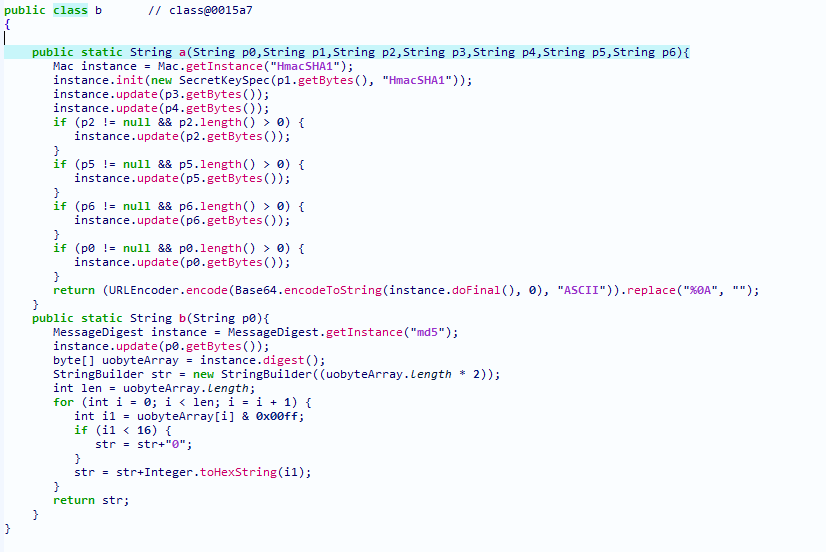
\includegraphics[width=0.7\textwidth]{images/pacer_gda2.png}
				\caption{Static method \textit{a} and method \textit{b}, of the class \textit{b}.}
			\end{figure}
			\par In this method a new instance of the object \textit{Mac} is retrieved with the method \textit{getInstance(''HmacSHA1'')}. This object is then initialized starting from the bytes relative to the second string passed as parameter. Then the object is updated with the bytes of other parameters. The return value is a \textit{Base64} encoding of the string obtained by the method \textit{doFinal} called on the Mac \textit{instance}, after having replaced the values \textit{''\%0A''} with \textit{''''}. This return value seems to assume the form of the value along the string \textit{Pacer}, in the \textit{Authorization} header. \newline
			Looking on the Java online documentation the class \textit{Mac} belongs to the library \textit{javax.crypto.Mac} and it provides the functionality for Message Authentication Code. In our case the \textit{''HmacSHA1''} standard algorithm is used.\newline
			At this point we are aware of the fact that some custom headers are used to compute the \textit{Authorization} header but we are only sure on few of them. More precisely the \textit{X-Pacer-Access-Token}, the \textit{X-Pacer-Time}, that represents the seconds from the Epoch, and \textit{X-Pacer-Nonce}, that is a random number generated between \textit{0} and \textit{1 bilion} (represented by \textit{0x3b9aca00} in hexadecimal). What it is not known yet are the \textit{p0, p1, p5, p6} values used in Figure 4.3. Going back in the code they belong to specific structures whose values can change at runtime.  \newline
			\par Instead of continuing with static analysis approach, I decided to approach the problem in a different way. Since the computation of the \textit{Authorization} header is done request by request, it should be possible to intercept the library calls for \textit{javax.crypto.Mac} and inspect the parameters passed to the methods directly at runtime. For this reason I used \textbf{Frida} for dynamic instrumentation purposes, explained in \ref{subsec:frida}.\newline
			\par I started creating a script able to intercept the two library calls \textit{javax.crypto.Mac} and \textit{javax.crypto.spec.SecretKeySpec}, overriding the definitions of the methods \textit{getInstance()}, \textit{init()}, \textit{update()} for the \textit{Mac} object, and also overriding the contructor for the object \textit{SecretKeySpec}. All the methods said above are substituded with new methods having the same semantic of the original ones, but just before returning the result they will print the the content of the parameters. Also a support function \textit{bin2String} has been implemented otherwise binary values will be printed instead of strings. The JavaScript code is embedded in a Python script that will handle the Frida process, attatching the script while spawing the process \textit{cc.pacer.androidapp}, as described in Section \ref{subsec:frida}. The final \textit{jscode} is the following:
\begin{lstlisting}
function bin2String(array) {
  var result = "";
  for (var i = 0; i < array.length; i++) {
    result += String.fromCharCode(array[i]);
  }
  return result;
}

const Mac = Java.use('javax.crypto.Mac');
const SecretKeySpec = Java.use('javax.crypto.spec.SecretKeySpec');

const Mac_getInstance = Mac.getInstance.overload('java.lang.String');
const Mac_init = Mac.init.overload('java.security.Key');
const Mac_update = Mac.update.overload('[B');
const SecretKeySpec_new = SecretKeySpec.$init.overload('[B', 'java.lang.String');

Mac_getInstance.implementation = function (str) {
	const result = Mac_getInstance.call(this, str);
	console.log('[+] Entering Mac.getInstance()');
	console.log('[ ] algo: ' + str);
	console.log('[-] Leaving Mac.getInstance()');
	console.log('');
	return result;
};

Mac_init.implementation = function (key) {
	const result = Mac_init.call(this, key);
	console.log('[+] Entering Mac.init()');
	console.log('[ ] key: ' + bin2String(key.getEncoded()));
	console.log('[-] Leaving Mac.init()');
	console.log('');
	return result;
};

Mac_update.implementation = function (bytes) {
	const result = Mac_update.call(this, bytes);
	console.log('[+] Entering Mac.update()');
	console.log('[ ] bytes: ' + bin2String(bytes));
	console.log('[-] Leaving Mac.update()');
	console.log('');
	return result;
}

SecretKeySpec_new.implementation = function (bytes, str) {
	const result = SecretKeySpec_new.call(this, bytes, str);
	console.log('[+] Entering SecretKeySpec()');
	console.log('[ ] bytes: ' + bin2String(bytes));
	console.log('[ ] algo: ' + str);
	console.log('[-] Leaving SecretKeySpec()');
	console.log('');
	return result;
}
\end{lstlisting}
			Of course we have no control on the runtime execution flow executed by the application, anyway from the previous investigation we know that everytime the application is opened, a POST request is issued to notify the server that Pacer passed to foreground. In the following output log it is possible to show the data associated to that request:
\begin{lstlisting}
[*] Running cc.pacer.androidapp

[+] Entering Mac.getInstance()
[ ] algo: HmacSHA1
[-] Leaving Mac.getInstance()

[+] Entering SecretKeySpec()
[ ] bytes: B7A4DB15-D69A-4C8A-BA68-39E0AA208DB8
[ ] algo: HmacSHA1
[-] Leaving SecretKeySpec()

[+] Entering Mac.init()
[ ] key: B7A4DB15-D69A-4C8A-BA68-39E0AA208DB8
[-] Leaving Mac.init()

[+] Entering Mac.update()
[ ] bytes: 1668595712
[-] Leaving Mac.update()

[+] Entering Mac.update()
[ ] bytes: 336394575
[-] Leaving Mac.update()

[+] Entering Mac.update()
[ ] bytes: pt_11b9df93-167d-4d31-b579-6a0cb2197f10
[-] Leaving Mac.update()

[+] Entering Mac.update()
[ ] bytes: app_version=p9.10.2&device_id=7021f2bad994fb65
[-] Leaving Mac.update()

[+] Entering Mac.update()
[ ] bytes: 84dfbceabc7185c5513137d08a431767
[-] Leaving Mac.update()

[+] Entering Mac.update()
[ ] bytes: /pacer/android/api/v18/accounts/334794565/actions/app_in_foreground
[-] Leaving Mac.update()
\end{lstlisting}
			The results obtained are the same obtained from the static analysis approach, but more accurated:
			\begin{enumerate}
			\item The method \textit{getInstance()} is called on the \textit{Mac} object with the string \textit{HmacSHA1} as parameter.
			\item A new \textit{SecretKeySpec} is created by passing a string \textit{p1} to it.  The \textit{p1} string is exactly \textit{''B7A4DB15-D69A-4C8A-BA68-39E0AA208DB8''}, and in the Figure 4.2 it is identified by the \textit{str3} variable: the one obtained from the \textit{Pedometer} object.
			\item The \textit{Mac} object is then initialized with the method \textit{init()} passing the string of the previous step.
			\item The method \textit{update()} on the \textit{Mac} object is called with the string \textit{''1668595712''}. This is the \textit{p3} variable representing the value of the \textit{X-Pacer-Time} header.
			\item The method \textit{update()} on the \textit{Mac} object is called with the string \textit{''336394575''}. This is the \textit{p4} variable representing the value of the \textit{X-Pacer-Nonce} header.
			\item The method \textit{update()} on the \textit{Mac} object is called with the string \textit{''pt\_11b9df93-167d-4d31-b579-6a0cb2197f10''}. This is the \textit{p2} variable representing the value of the \textit{X-Pacer-Access-Token} header.
			\item The method \textit{update()} on the \textit{Mac} object is called with the string \newline
			\textit{''app\_version=p9.10.2\&device\_id=7021f2bad994fb65''}. This is the \textit{p5} variable, relative to the \textit{str2} variable in Figure 4.2. This is the value obtained from the \textit{ot} object.
			\item The method \textit{update()} on the \textit{Mac} object is called with the string \textit{''84dfbceabc7185c5513137d08a431767''}. This is the \textit{p6} variable, relative to the \textit{str5} variable in Figure 4.2. This is the value obtained from \textit{this} object, applying the method \textit{a}. This string really seems to be an hash digest of some value. As showed in Figure 4.3 there is another method not yet used. The routine is similar to the one just described, but with just a single string as parameter, and uses the \textit{MD5} algorithm. It is not hard to guess that this is the MD5 hash value of the body of the request. It is easy to double check with any MD5 online hash tool.
			\item The method \textit{update()} on the \textit{Mac} object is called with the string \textit{''/pacer/android/api/v18/accounts/334794565/actions/app\_in\_foreground''}. This is the \textit{p0} variable, relative to the \textit{path} parameter in Figure 4.2. This is the value obtained from the \textit{ot} object with the methods \textit{F()} and \textit{getPath()}.
			\end{enumerate}
			With a dynamic instrumentation approach we got all the values used at runtime by the code showed in Figure 4.2. Anyway we are not sure that the final string computed is actually used as \textit{Authorization} header. \newline
			\par To prove the concept just explained, I created a Java program with the same first method showed in Figure 4.3. The code is reported below:

\begin{lstlisting}
public static String foo(String p0,String p1,String p2,String p3,String p4,String p5,String p6) throws NoSuchAlgorithmException, InvalidKeyException, UnsupportedEncodingException{

Mac instance = Mac.getInstance("HmacSHA1");
instance.init(new SecretKeySpec(p1.getBytes(), "HmacSHA1")); // PEDOMETER ID
instance.update(p3.getBytes());                            		// TIME
instance.update(p4.getBytes());                     			// NONCE
if (p2 != null && p2.length() > 0) {           					// ACCESS_TOKEN
	instance.update(p2.getBytes());
}
if (p5 != null && p5.length() > 0) {         // PATH PARAMETERS
	instance.update(p5.getBytes());
}
if (p6 != null && p6.length() > 0) {      // MD5 BODY (POST, PUT, PATCH)
	instance.update(p6.getBytes());
}
if (p0 != null && p0.length() > 0) {          // URL PATH
	instance.update(p0.getBytes());
}
return (URLEncoder.encode(Base64.encodeToString(instance.doFinal(), 0), "ASCII")).replace("%0A", "");
}
    
public static void main(Strings[] args) {
	String p0, p1, p2, p3, p4, p5, p6;
	p0 = "/pacer/android/api/v18/accounts/334794565/actions/app_in_foreground"; // p0.i.F.getPath();
	p1 = "B7A4DB15-D69A-4C8A-BA68-39E0AA208DB8"; 	//Pedometer.o(...)  
	p2 = "pt_11b9df93-167d-4d31-b579-6a0cb2197f10"; 		//"X-Pacer-Access-Token";
	p3 = "1668595712";  //"X-Pacer-Time" 
	p4 = "336394575";   //"X-Pacer-Nonce" 
	p5 = "app_version=p9.10.2&device_id=7021f2bad994fb65"; // Path parameters;
	p6 = "84df-bceabc7185c5513137d08a431767"; //  md5 body

	String ret = null;
	try {
		ret = foo(p0, p1, p2, p3, p4, p5, p6);
	} catch (NoSuchAlgorithmException e) {
		e.printStackTrace();
	} catch (InvalidKeyException e) {
		e.printStackTrace();
	} catch (UnsupportedEncodingException e) {
		e.printStackTrace();
	}

	System.out.println(ret);
}
\end{lstlisting}
			\par The \textit{foo} function is copy-pasted from the Figure 4.3, while the values of the parameters are directly typed in the code. Any test can be done with any request showed in HttpToolkit. The fields needed for the computation of the \textbf{Authorization header} are \textbf{URL Path}, \textbf{X-Pacer-Access-Token}, \textbf{X-Pacer-Time}, \textbf{X-Pacer-Nonce}, \textbf{URL Parameters}, \textbf{MD5 Body Hash}, and \textbf{Pedometer Code} (a value constant for the whole installation of the Pacer application. 
		
		\subsubsection{Testing unauthorized access \#2}
			\par Now that we have achieved to forge the Authorization header, we know that in the previous test there was something wrong. Indeed we were modifying the \textit{URL path} (changing the target resource) without changing the value of the \textit{Authorization} header. Using our Java program to forge this header the values to use are:
			\begin{itemize}
				\item p0 = "/pacer/android/api/v18/accounts/334794565'', that is the \textit{URL path}.
				\item p1 = "B7A4DB15-D69A-4C8A-BA68-39E0AA208DB8", that is the \textit{Pedometer code}.
				\item p2 = "pt\_ade60014-e7a8-4b96-9fc0-0bf7cfeaf983", that is the \textit{"X-Pacer-Access-Token"} header.
				\item p3 = "1675465946", that is the \textit{"X-Pacer-Time"} header.
				\item p4 = "302363282", that is the \textit{"X-Pacer-Nonce"} header.
				\item p5 = "". There are no parameters needed for this URL.
				\item p6 = "". Body not handled by the application in GET requests.
			\end{itemize}
			The value returned from our program is \textit{Lgm4YH\%2Bthm3zl5NtfCadLgsy6Ho\%3D}. This will be the value to use for the \textit{Authorization} header.\newline
			Proceeding by forging the request in BurpSuite this is what we obtain:
			\begin{figure}[ht]
				\centering
				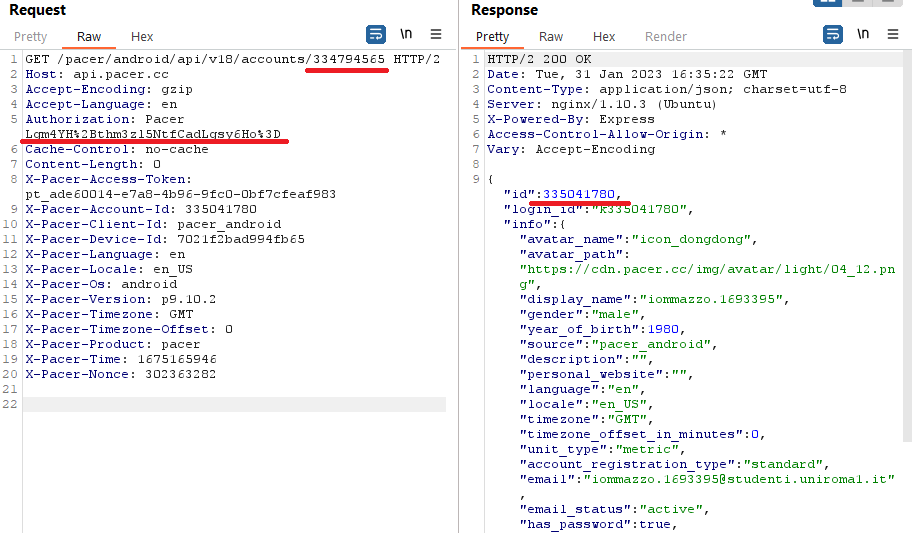
\includegraphics[width=\textwidth]{images/pacer3.png}
				\caption{Test request \#2.}
			\end{figure}
			\newpage
			\par There is no error message showed, meaning that the \textit{Authorization} header we computed it is correct. Anyway the response is not the one we were expecting. Even if the resource on which the GET is performed is the one linked to my personal email (account id \textit{334794565}), the response data retrieved are those relatives to the account we are actually using (account id \textit{335041780}). It is a unexpected behaviour, meaning that the resource specified in the url path is ignored. Indeed a different value is specifying the resource retrieved.
			
		\subsubsection{Testing unauthorized access \#3}
			\par Looking at the forged request, the discriminant value, specifiying on which account we are retrieving informations on, has to be the \textbf{X-Pacer-Account-Id}. In the previous request it was still set to the account id linked to the institutional email. \newline
			The \textit{Authorization} header is not affected by this change, so we can simply change this value to \textit{334794565}, the \textit{pacer\_id} of the account we want to retrieve information on.
			\newpage
			\begin{figure}[ht]
				\centering
				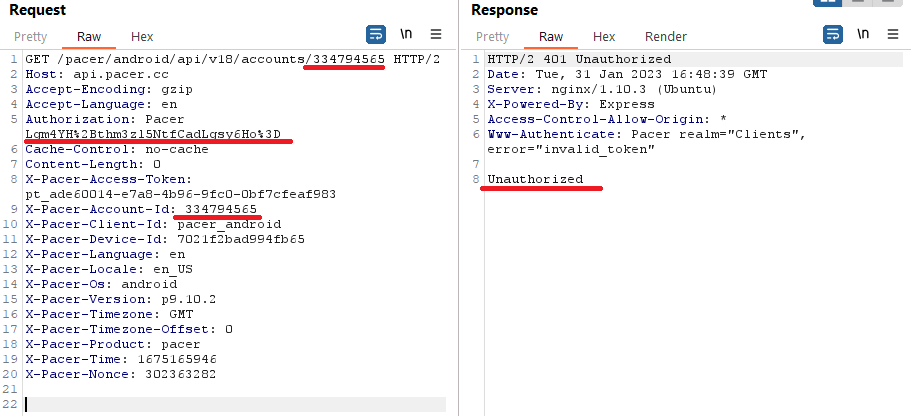
\includegraphics[width=\textwidth]{images/pacer4.png}
				\caption{Test request \#3.}
			\end{figure}
			\par Finally we get an \textit{Unauthorized} message from the server. We have almost checked all the custom headers available. The response \textit{Www-Authenticate} header is saying \textit{error=''invalid\_token''}. Definitely the \textit{X-Pacer-Access-Token} we are using is not providing us with enough permissions to access informations related to other accounts. 
			
		\subsubsection{X-Pacer-Access-Token}
			\par We already have met this token while forging the \textit{Authorization} header. In any case going back in the communication protocol, I started analyzing all the requests generated in order to understand where this access token is obtained from. This token is assigned at the moment of the user login, after having sent the fields \textit{email} and \textit{password}, or after having completed the OAuth procedure to log in with Facebook or Google. In order to test this behaviour and investigate those requests in HttpToolkit I performed a logout, and again a login on the same account with id \textit{335041780}. \newline
			These are four moments in which the investigation has been performed: during the first request generated without any access token, before the login, during the login action, and after the login:\newpage
			\begin{figure}[ht]
				\centering
				\subfigure[First request]{
				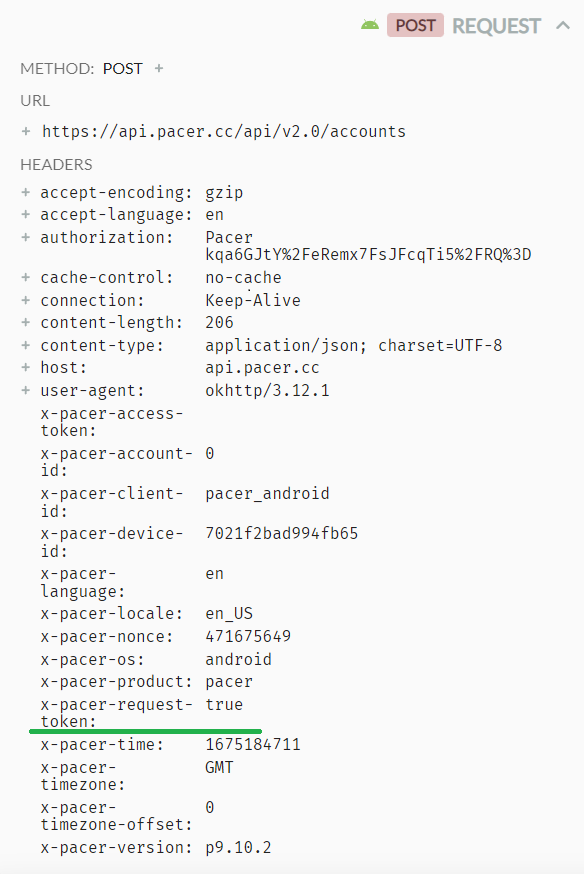
\includegraphics[width=.35\textwidth]{images/pacer_login_1.png}
				}
				\subfigure[Before login requests]{
				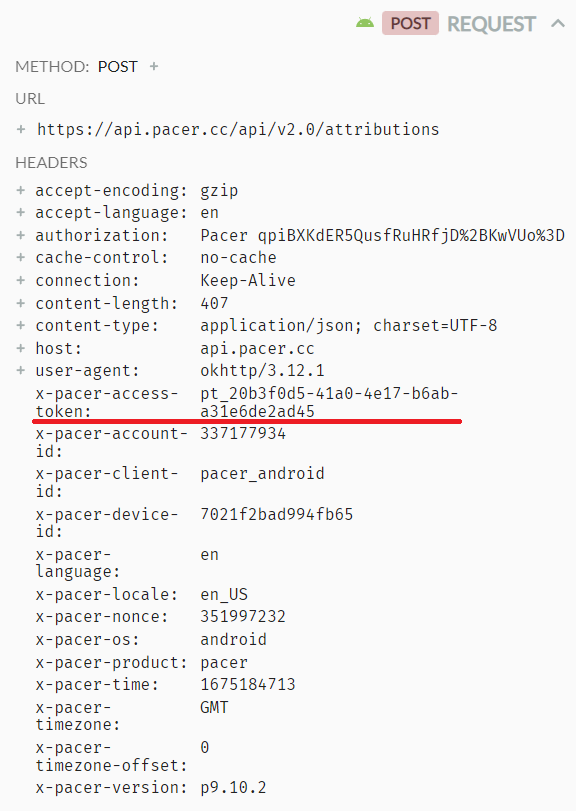
\includegraphics[width=.35\textwidth]{images/pacer_login_2.png}
				}
				\hfill
				\subfigure[Login request]{
				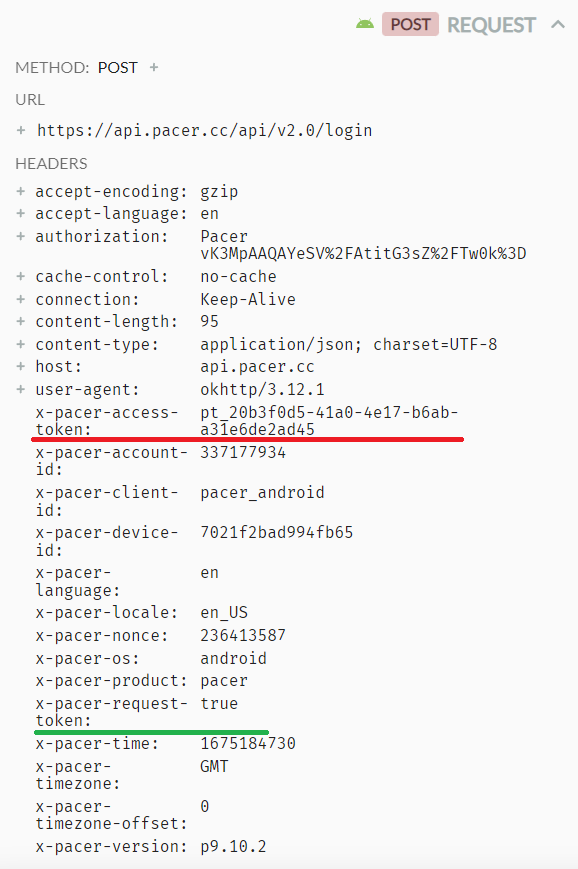
\includegraphics[width=.35\textwidth]{images/pacer_login_3.png}
				}
				\subfigure[After login requests]{
				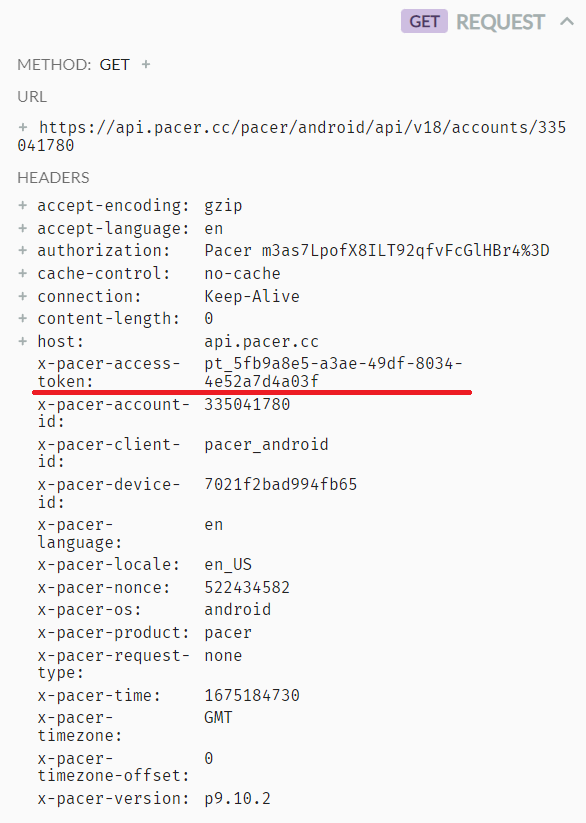
\includegraphics[width=.35\textwidth]{images/pacer_login_4.png}
				}
				\caption{X-Pacer-Access-Token investigation}
			\end{figure}
			\par	During the first request [Figure (a)] the POST request has no access token. In this moment the client is actually asking the server for a new one, in fact the header \textbf{X-Pacer-Request-Token} is set to \textit{true}. The response to this request contains a fresh access token, to use in the pre-login phase. \newline
			Before the user actually logs in [Figure (b)] the \textit{X-Pacer-Access-Token} used is the one retrieved from the previous step. \newline
			While performing the \textit{login} [Figure (c)] a POST request is issued communicating \textit{email} and an hash digest of the \textit{password}. The access token used is still the one received at the previous step. Anyway after the login we will need a new access token, associated instead with the account just logged in. Even in this case then the \textbf{X-Pacer-Request-Token} is set to \textit{true}. The response to this login request contains the actual access token.
			After having performed the login action [Figure (d)] the \textit{X-Pacer-Access-Token} assume the value obtained from the login response. From this moment going on, the value of the access token will be this one for every request.\newline
			Investingating the different log in phases a new header is discovered: the \textbf{X-Pacer-Request-Token}. Clearly it is used when the client is requesting a new access token, exactly in the Figures (a) and (c).
			
		\subsubsection{Final unauthorized access }
			\par Now that I have known about this new header \textbf{X-Pacer-Request-Token}, I have tryed to forge a request, still having the \textit{X-Pacer-Access-Token} set as standard, but adding a new header that is the \textit{X-Pacer-Request-Token}. If by any chance this last header is being evaluated without actually checking the \textit{X-Pacer-Access-Token} we might bypass any authorization mechanism tied to the access-token. This is the request forged: 
			\begin{figure}[ht]
				\centering
				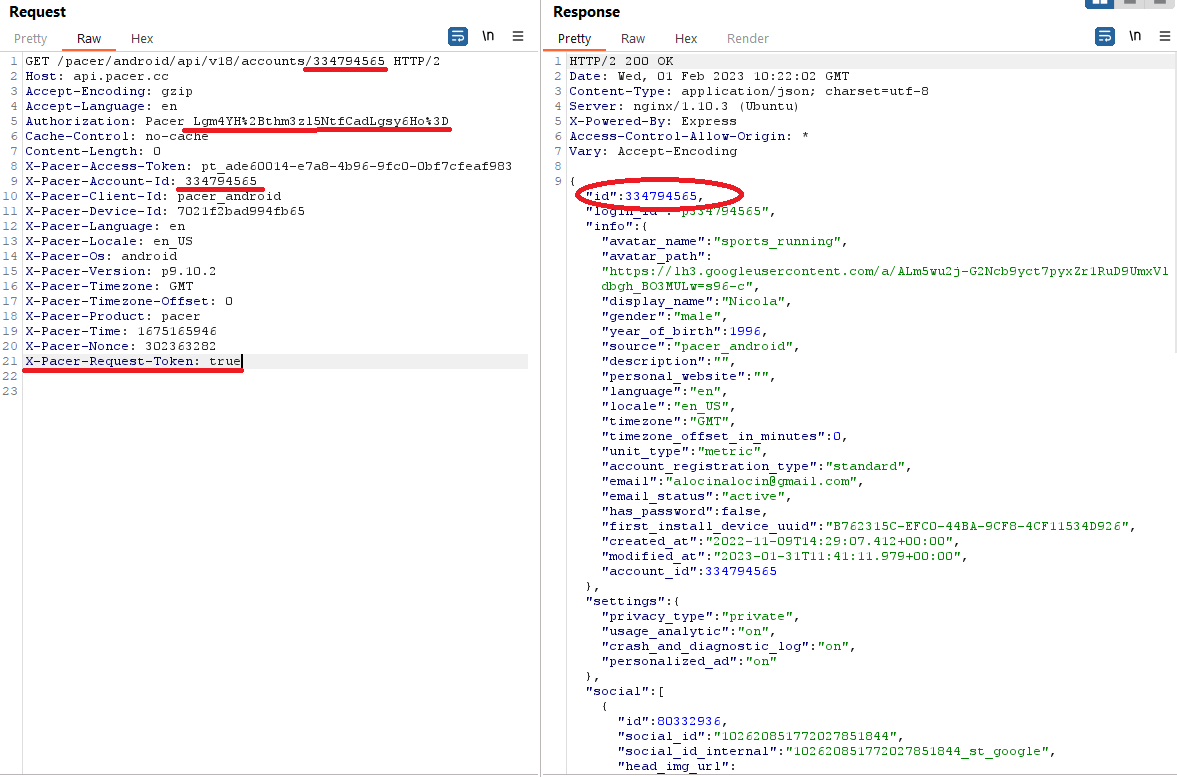
\includegraphics[width=0.9\textwidth]{images/pacer5.png}
				\caption{Test request \#4.}
			\end{figure}
			\par Here we go. The response showed on the right side of the picture contains information about my personal account (id \textit{334794565}) comprensihive of email, gender, picture, social media identifiers. Notice that this is not the case in which I am visiting another user profile, that is a legit action to perform in Pacer: I could have simply visit the account id \textit{334794565}, but the informations retrieved do not contains any personal informations, as showed in the Accessing Resource paragraph of this Section. With this procedure we are asking to the server informations on an account, that we do not actually own, as owner of that account. It is clearly something that should not happen.\newline
			Moreover combining this last \textbf{X-Pacer-Request-Token}, with the forge of the \textbf{Authorization} header described above, we are literally able to control another account as we were its owner and without needing the access credentials.
			
		\subsubsection{Changing setting of another user account}
			\par In this paragraph we will push the investigation beyond the scope of accessing the resources. I already have shown how informations can be retrieved on an account that we do not own. Since the \textit{X-Pacer-Request-Type} let us to access information otherwise not accessible, and the \textit{Authorization} header let us to visit every path explorable in the server, why not to try if we can actually forge some POST request, for example modifying to settings relative an another account.\newline
			\par The setting chosen to work on is the Privacy value of an account. On most social platforms an user can decide if its account is \textit{private}, meaning that the informations tied to his account are visible only to his friends, or \textit{public}, meaning that every user can view its informations. Thanks to HttpToolkit, and simulating this setting changing on the emulator, we identified the POST request to be directed towards the resource \textit{/api/v2.0/accounts/<pacer\_id>/settings/<section>}, where \textit{<pacer\_id>} is the target id account (in this case our target account is \textit{334794565}), and \textit{<section>} can assume one of this values [\textit{gps}, \textit{privacy}, \textit{workout}], defining the section of the settings we are going to modify. \newline
			The url path is given. The forged request will have the following headers:
			\begin{enumerate}
				\item \textit{X-Pacer-Access-Token} is the one of our account.
				\item \textit{X-Pacer-Request-Token} set to \textit{true}, this will bypass the check on the access token.
				\item \textit{X-Pacer-Nonce}: we can use the older values for the nonce.
				\item \textit{X-Pacer-Time}: we can use the older values for the time.
				\item \textit{X-Pacer-Account-Id}: we can leave this value to the target id account, and see how it works.
				\item Every other \textit{X-Pacer} header can be left as it was.
				\item Since this is a POST request there will be also a body. In this case the body of the request will contain the whole list of settings belonging to the section Privacy. From HttpToolkit we know that the body is a JSON structure of the form:
\begin{lstlisting}
{"crash_and_diagnostic_log":null,"personalized_ad":null,"privacy_type":"public","usage_analytic":null}
\end{lstlisting}
				\par where the specific setting values we are going to change have to be set, while every other value is not changed is \textit{null}. Since on our target account the privacy setting is set to \textit{''private''},	try instead to change it in \textit{''public''}.
				\item Finally the \textit{Authorization} header has to be forged with our Java program, keeping in considerations the values of \textit{url path}, \textit{Pedometer code} (still the same leaked with Frida), \textit{X-Pacer-Access-Token}, \textit{X-Pacer-Time}, \textit{X-Pacer-Nonce}, \textit{path parameters} (there are no parameters for this requests), \textit{MD5 of body request}. We already got all of these value. We only miss the \textit{MD5} hash of the body, easily computable with any MD5 online tool. In this case the hash digest of the body is \textit{34303e67eaa68ec11ab5c6556c74f9e4}. The resulting \textit{Authorization} header is \textit{lXT8UuMb\%2F49KgK8ZRCAloUoPbV4\%3D}.
			\end{enumerate}
			\par The request and response generated with in BurpSuite are:\newpage
			\begin{figure}[ht]
				\centering
				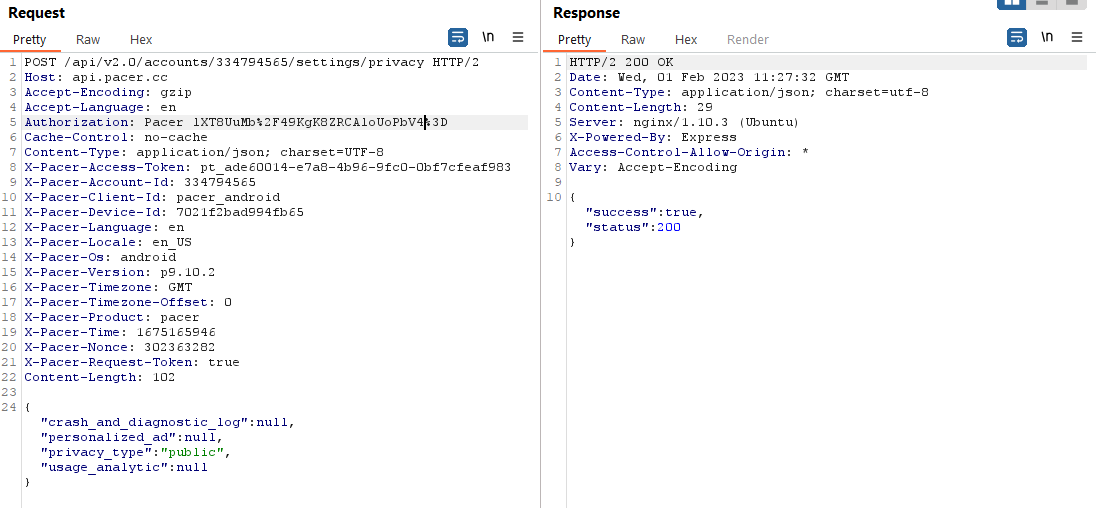
\includegraphics[width=\textwidth]{images/pacer_privacy.png}
				\caption{Privacy setting change request.}
			\end{figure}
			\par The response expresses that the request was successful. \newline
			By comparing the informations retrieved on the target account before and after our forged POST, we can see the differences:
			\begin{figure}[ht]
				\centering
				\subfigure[Before the POST request]{
				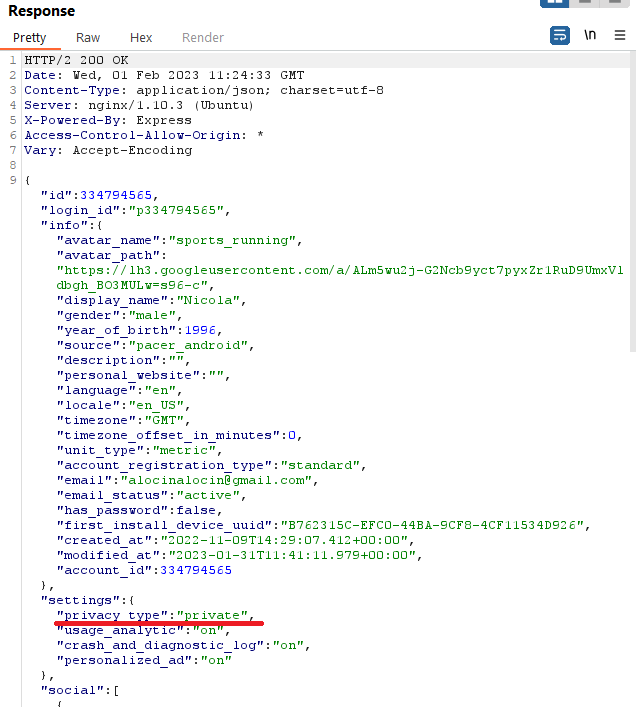
\includegraphics[width=.45\textwidth]{images/pacer6.png}
				}
				\subfigure[After the POST request]{
				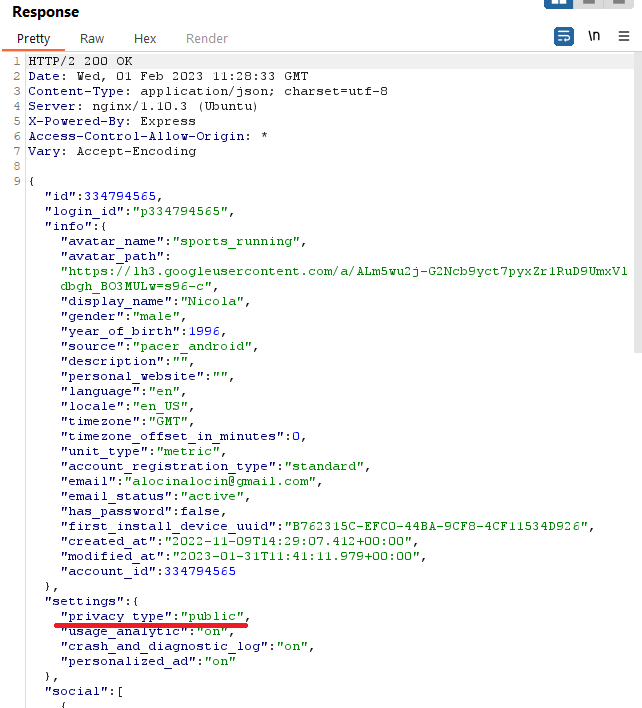
\includegraphics[width=.45\textwidth]{images/pacer7.png}
				}
				\caption{Before and after the privacy settings change}
			\end{figure}
			\par The procedure described was actually able to change the privacy settings of a target account, by only knowing its \textit{pacer\_id}. \newline
			\par The procedure is therefore valid for every other kind of settings change.
			
			\subsubsection{Training paths}
				\par Keep going with the private informations investigation, another feature of the Pacer application has been analyzed, that is the \textit{Training Paths} sharing. Each user can record its training session and save the log of the session, comprehensive of calories, distance, and time the session lasted. The application handle two types of training paths:
				\begin{enumerate}
					\item \textit{Locally stored training paths}: Every training routine manually started by the user will be saved offline on the device, and it is possible access it only from the device that logged that training session. \newline
					\item \textit{Public shared training paths}: The locally stored sessions can be chosen to be publicly shared. These ones are accessible from the \textit{Feed} tab by any user following our account, from the \textit{Explore} tab by a user that is near the location of the training path, or by visiting the user profile.
				\end{enumerate}
				\par The first type of training paths cannot be inspected without a physical access to the device. On the other way the second ones are accessible, in fact the user that published them have decided to share it with the community. In this sense there is no actual leak of private informations obtainable from these, since the user has spontaneously chosen to share them.
				
			\subsubsection{Obtaining user account IDs}
				\par Up to now we only miss a single component in order to retrieve personal data on a target user, that is its \textit{account\_id}. As introducted before, Pacer in the \textit{Explore} tab of the application, provide a map where it is possible to visualize the training paths published by the users. Tapping on one of these paths the informations on the path and on the users that used that paths as training route are shown. In the Pacer application are not directly visible the users \textit{account\_id}, but on the HTTPS response they are. The following picture shows both the Pacer application view and the relative body HTTPS response:\newpage
			\begin{figure}[ht]
				\centering
				\subfigure[Pacer application response view]{
				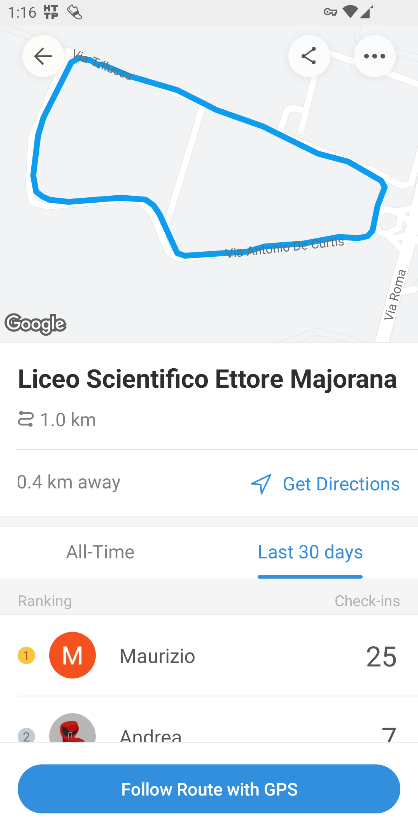
\includegraphics[width=.35\textwidth]{images/pacer_path_1.png}
				}
				\subfigure[HTTPS response]{
				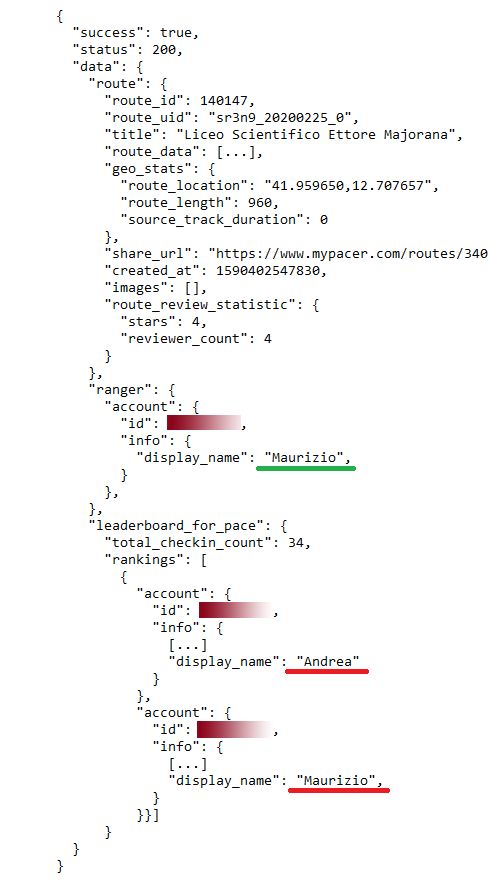
\includegraphics[width=.35\textwidth]{images/pacer_path_2.png}
				}
				\caption{Visiting a path from the Explore tab of the application}
			\end{figure}
			
				\par As the picture (a) describes, from the Pacer application can only be seen which are the top ranked users. Even by tapping on a profile the relative \textit{account\_id} is not shown. On the right side picture (b) it is indeed showed the JSON code in the body of the HTTPS response, in a redacted form and obscurated from the \textit{id\_account} of the relative users. The first one is the creator of the route, while the below ones are from the ranking list. \newline
				\par This is only a possible way of retrieving \textit{account\_id} values of the Pacer user. In fact every comment and post from the \textit{Explore} and \textit{Feed} tabs in the Pacer application will deliver us the \textit{account\_id} of the user. Once obtained the user account id, the whole procedure for accessing other users resources described above can be achieved.
				
	\subsection{Results}
		\par Here are reported the results obtained by the Pacer application study case.
		
		\subsubsection{Private informations leaked}
		\par The Pacer application is exposed to users private informations leak. Given a Pacer user \textit{account\_id} it is possible to obtain the following private informations:
		\begin{itemize}
			\item Profile picture.
			\item Gender.
			\item Email address.
			\item Device UUID.
			\item Country and Timezone.
			\item Facebook and Google social data linked including:
			\begin{itemize}
				\item Social nickname.
				\item Social profile picture.
				\item Social ID used for the Pacer app.
			\end{itemize}
		\end{itemize}

		\subsubsection{Other vulnerabilities}
			\par The study conducted shows the presence of an important vulnerability that allows an user to bypass the access-token based authorization mechanism, and access the private resources of any Pacer \textit{account\_id} user. \newline
			This vulnerability exploitation might bring to the loss of control for any user on its own account. Any account can be accessed by simply having the relative \textit{account\_id}. \newline
			The source of the vulnerability relies in how the back-end system handle the header \textit{X-Pacer-Request-Token}.
		
\newpage